%%%%%%%%%%%%%%%%%%%%%%%%%%%%%%%%%%%%%%%%%
% University/School Laboratory Report
% LaTeX Template
% Version 3.0 (4/2/13)
%
% This template has been downloaded from:
% http://www.LaTeXTemplates.com
%
% Original author:
% Linux and Unix Users Group at Virginia Tech Wiki 
% (https://vtluug.org/wiki/Example_LaTeX_chem_lab_report)
%
% License:
% CC BY-NC-SA 3.0 (http://creativecommons.org/licenses/by-nc-sa/3.0/)
%
%%%%%%%%%%%%%%%%%%%%%%%%%%%%%%%%%%%%%%%%%

%----------------------------------------------------------------------------------------
%	PACKAGES AND DOCUMENT CONFIGURATIONS
%----------------------------------------------------------------------------------------

\documentclass{article}

\usepackage[version=3]{mhchem} % Package for chemical equation typesetting
\usepackage{siunitx} % Provides the \SI{}{} command for typesetting SI units

\usepackage[top=1in, bottom=1in, right=1in, left=1in]{geometry}

%Add code formating
\usepackage{listings}
\lstset{tabsize=2}

\usepackage{hyperref}

\usepackage{amssymb}

\usepackage{enumerate}

%Add extra support for image placement
\usepackage{float}

\usepackage{mcode}

\usepackage{graphicx} % Required for the inclusion of images

\setlength\parindent{0pt} % Removes all indentation from paragraphs

\renewcommand{\labelenumi}{\alph{enumi}.} % Make numbering in the enumerate environment by letter rather than number (e.g. section 6)

%\usepackage{times} % Uncomment to use the Times New Roman font

%----------------------------------------------------------------------------------------
%	DOCUMENT INFORMATION
%----------------------------------------------------------------------------------------

\title{Keysight Hacking Platform Getting Started} % Title

\author{Blake \textsc{Vermeer}} % Author name

\date{\today} % Date for the report

\begin{document}

\maketitle % Insert the title, author and date

\begin{center}
\begin{tabular}{l r}
Date Performed: & March 21, 2017 \\ % Date the experiment was performed
Company: & Keysight Technologies % Company
\end{tabular}
\end{center}

% If you wish to include an abstract, uncomment the lines below
% \begin{abstract}
% Abstract text
% \end{abstract}

%----------------------------------------------------------------------------------------
%	OVERVIEW
%----------------------------------------------------------------------------------------
\section{Overview}

The Keysight Hacking Platform is designed to have a development workflow similar to how firmware is developed in most Keysight products while yet at the same time being flexible enough that students can develop their own software / hardware for a Hackathon. \\

The Keysight Hacking Platform consists of:

	\begin{itemize}
		
		\item Raspberry Pi 3 with 2.8" capacitive touch screen shield
		
		\item Custom Yocto Linux image pre-loaded on the Raspberry Pi 3
		
		\item Fedora Linux Virtual Machine image with Qt Creator and the Yocto SDK pre-installed and configured with Qt Creator
		
	\end{itemize}

The general workflow for creating applications using the KHP is the application is created in the Qt Creator program that is pre-installed in the virtual machine image. The application is then cross-compiled by Qt Creator using the Yocto SDK and is then sent over WiFi to the Raspberry Pi where the application is run and can be debugged remotely using Qt Creator.

	\begin{figure}[H]
		\centering
		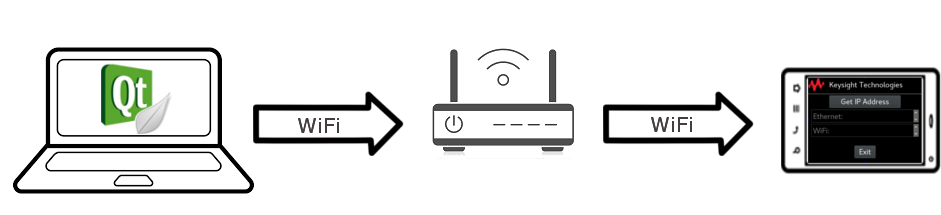
\includegraphics[scale=0.5]{pics/Deployment_Workflow.png}
		\caption{Qt App Deployment Workflow}
		\label{Qt_App_Deployment}
	\end{figure}



%----------------------------------------------------------------------------------------
%	Installing VirtualBox
%----------------------------------------------------------------------------------------
\section{Installing VirtualBox}

To be able to use the pre-setup virtual machine image you must first install VirtualBox. Go to the subsection below for your OS and follow the directions.


	\subsection{Windows}
	
	Go to the VirtualBox download location \href{https://www.virtualbox.org/wiki/Downloads}{VirtualBox Download} and click the link for "Windows hosts." After downloading the installer run it and follow the prompts.
	
	\subsection{Mac}
	
	Go to the VirtualBox download location \href{https://www.virtualbox.org/wiki/Downloads}{VirtualBox Download} and click the link for "OS X hosts." After downloading the installer run it and follow the prompts.
	
	\subsection{Linux}
	
	VirtualBox is available in most Linux distributions package managers. Install VirtualBox through the package manager for your particular Linux distribution. If VirtualBox is not available in your Linux distribution's package manager, VirtualBox provides pre-build binaries for various Linux distributions. More information is available at this link: \href{https://www.virtualbox.org/wiki/Linux_Downloads}{VirtualBox Linux Downloads}.



%----------------------------------------------------------------------------------------
%	Importing the Virtual Machine
%----------------------------------------------------------------------------------------
\section{Import the Virtual Machine}

After install VirtualBox, the next step is to import the virtual machine image into VirtualBox. After starting up VirtualBox, choose \textbf{Import Appliance...} from the file menu.

	\begin{figure}[H]
		\centering
		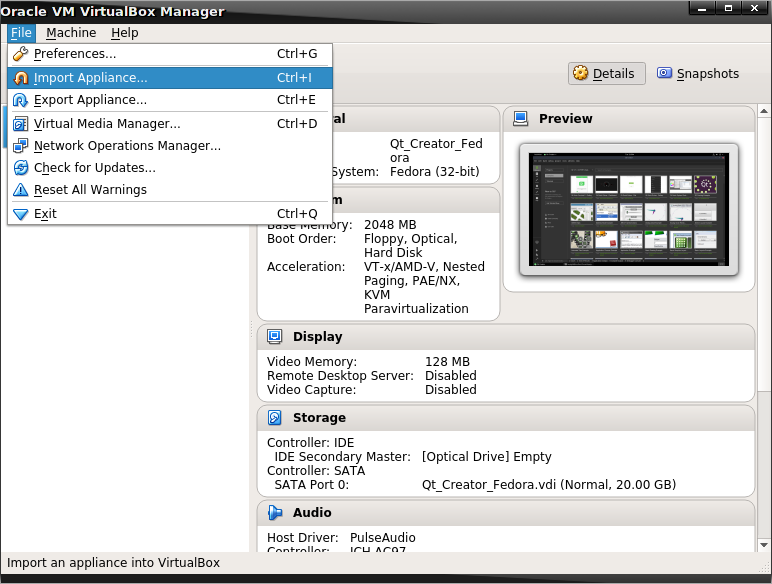
\includegraphics[scale=0.35]{pics/VirtualBox_Import_Appliance.png}
		\caption{Import Virtual Machine}
		\label{Import_Virtual_Machine}
	\end{figure}


Navigate to the location of the virtual machine image (Qt\_Creator\_Fedora.ova) and then click next. 


	\begin{figure}[H]
		\centering
		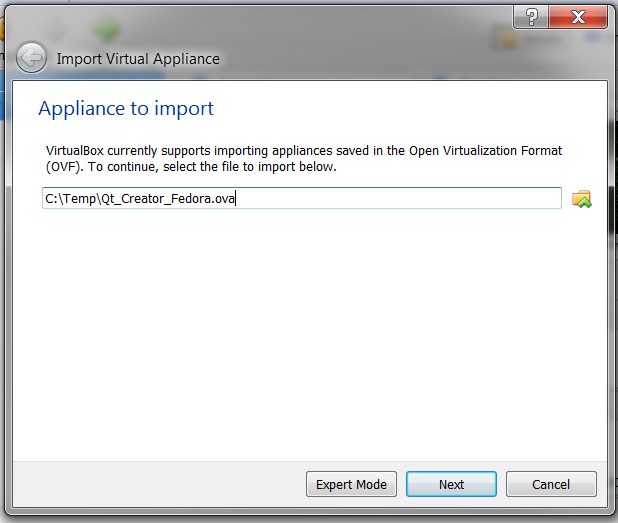
\includegraphics[scale=0.75]{pics/VirtualBox_VM_Location.png}
		\caption{Locate the Virtual Machine}
		\label{Locate_Virtual_Machine}
	\end{figure}


In the next screen that appears (Appliance settings) make sure to click the checkbox to reinitialize the MAC addresses of all the network cards.


	\begin{figure}[H]
		\centering
		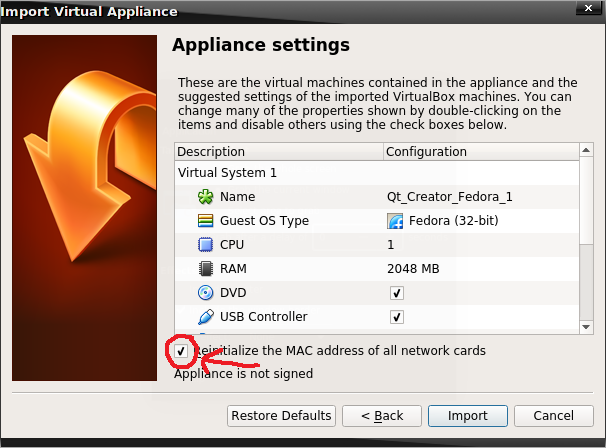
\includegraphics[scale=0.75]{pics/VirtualBox_Appliance_Settings.png}
		\caption{Import Virtual Machine Settings}
		\label{Import_Virtual_Machine_Settings}
	\end{figure}

After importing the virtual machine image, the main VirtualBox screen should appear similar to Figure \ref{VirtualBox_Main_Window}. To start the virtual machine, highlight the \textbf{Qt\_Creator\_Fedora} virtual machine from the list and then click the start button.

	\begin{figure}[H]
		\centering
		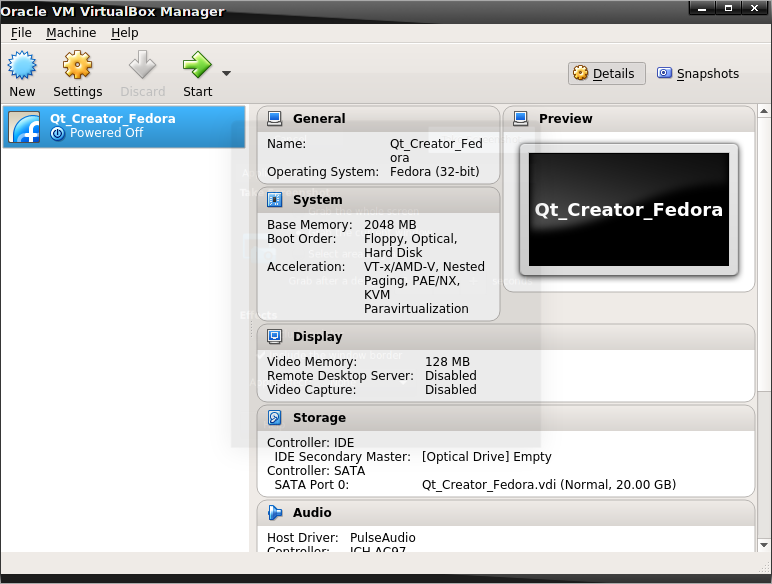
\includegraphics[scale=0.35]{pics/VirtualBox_Main_View.png}
		\caption{VirtualBox Main Window}
		\label{VirtualBox_Main_Window}
	\end{figure}


%----------------------------------------------------------------------------------------
%	Log into the Virtual Machine
%----------------------------------------------------------------------------------------
\section{Log into the Virtual Machine}

After starting the virtual machine and waiting for it to boot, you will be presented with the login screen. Press enter and enter "keysight" for the password.

	\begin{figure}[H]
		\centering
		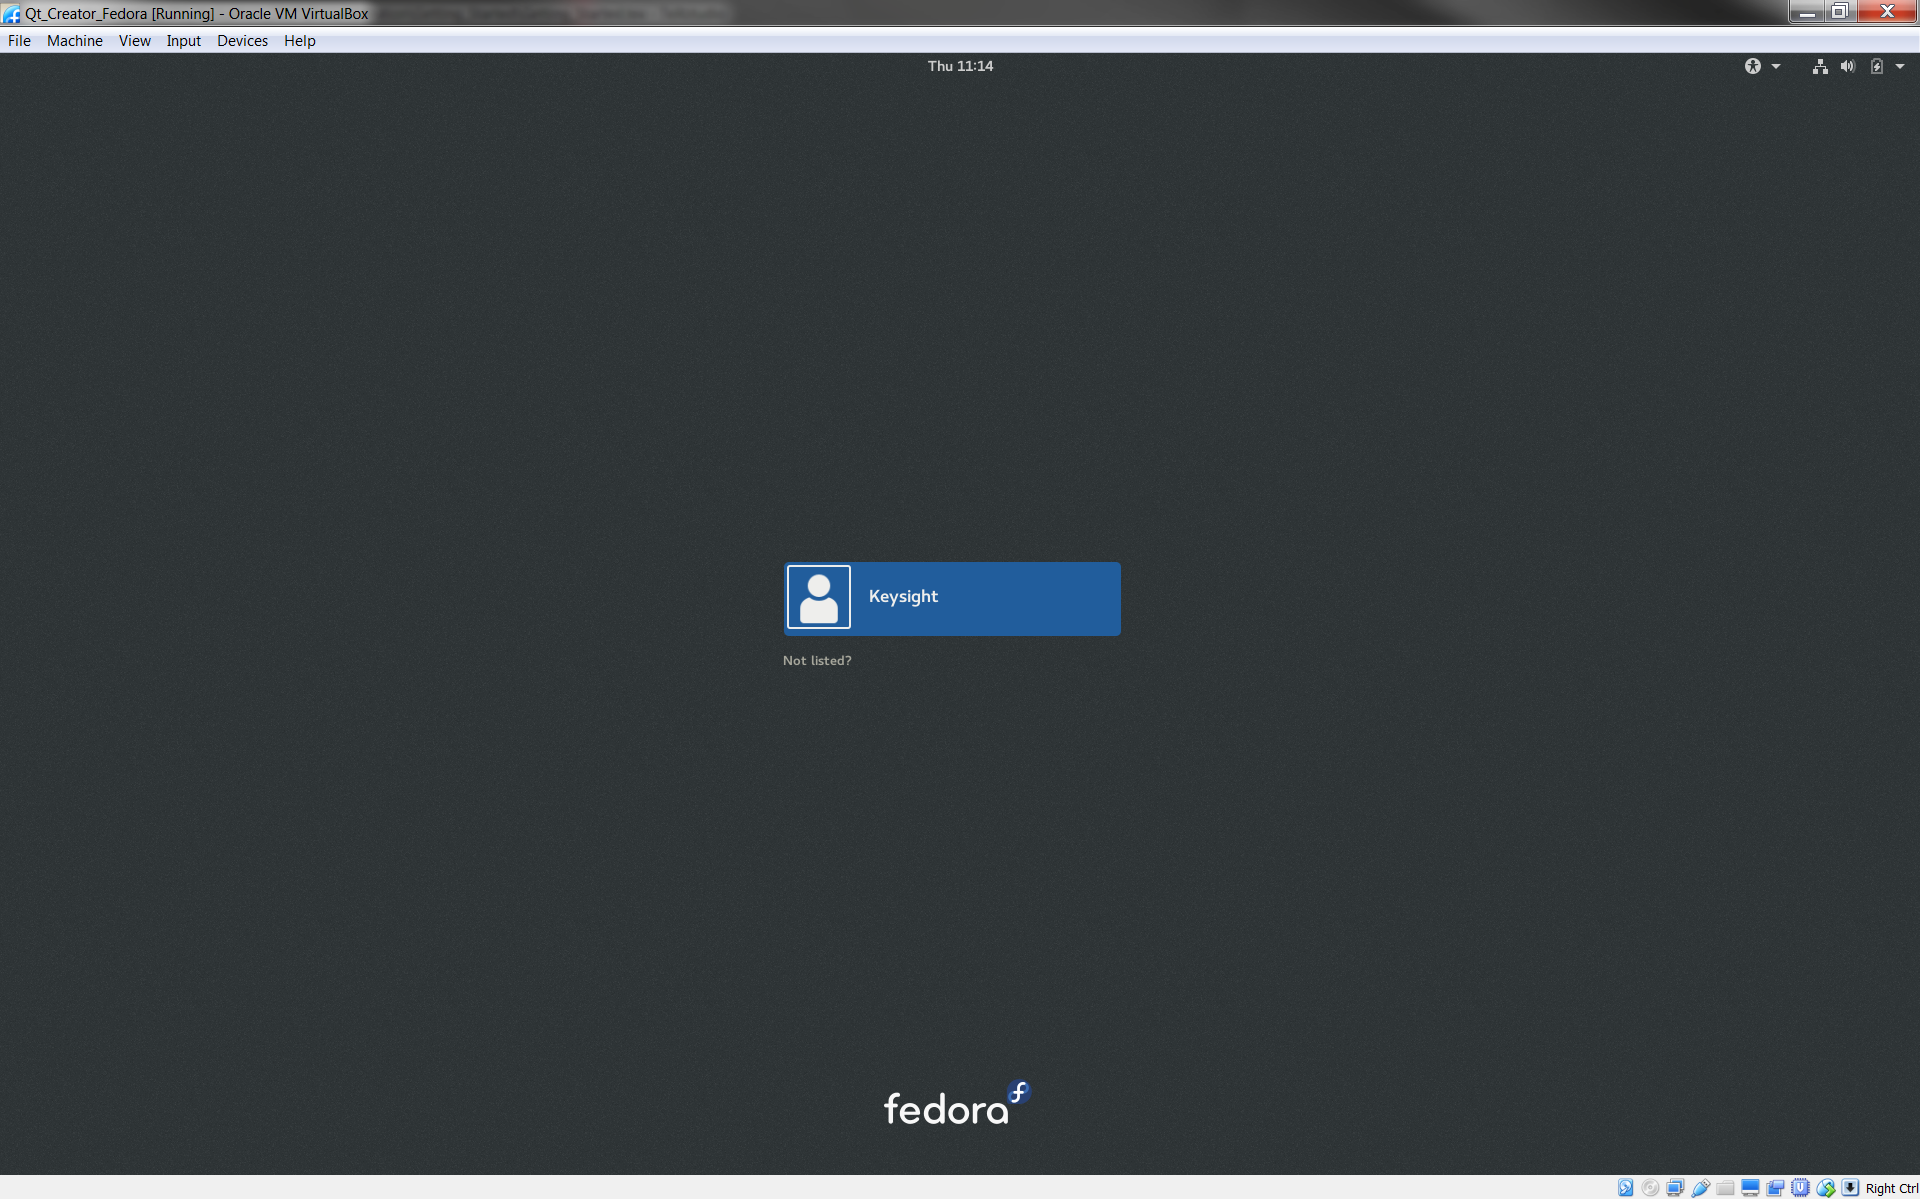
\includegraphics[scale=0.25]{pics/VM_Login.png}
		\caption{Virtual Machine Login (the password is: "keysight")}
		\label{VM_login}
	\end{figure}

Next the desktop will appear. Double-click on the Qt Creator icon to start Qt Creator.

	\begin{figure}[H]
		\centering
		
\includegraphics[scale=0.35]{pics/VM_Desktop.png}
		\caption{Virtual Machine Desktop}
		\label{VM_desktop}
	\end{figure}

%----------------------------------------------------------------------------------------
%	Connect the Raspberry Pi to Qt Creator
%----------------------------------------------------------------------------------------
\section{Connect the Raspberry Pi to Qt Creator}

After starting Qt Creator, the first step is to connect the Raspberry Pi to Qt Creator. To do this first power on the Raspberry Pi and wait for the Keysight show IP program to start. Click the \textbf{Get IP Address} button to show the configured IP address for the ethernet and WiFi interfaces. Depending on how quickly the interface receives an IP address you may have to click the button a few times.

	\begin{figure}[H]
		\centering
		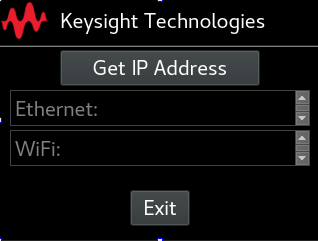
\includegraphics[scale=0.75]{pics/Show_IP_app.png}
		\caption{Keysight Show IP App}
		\label{Show_IP_app}
	\end{figure}

Write down the IP address of the interface you would like to use. In the Qt Creator program go to the \textbf{Tools} $\Rightarrow$ \textbf{Options} dialog box. In the \textbf{Options} dialog box go to the \textbf{Devices} tab. In the \textbf{Host Name} field, enter the IP address of the Raspberry Pi.


	\begin{figure}[H]
		\centering
		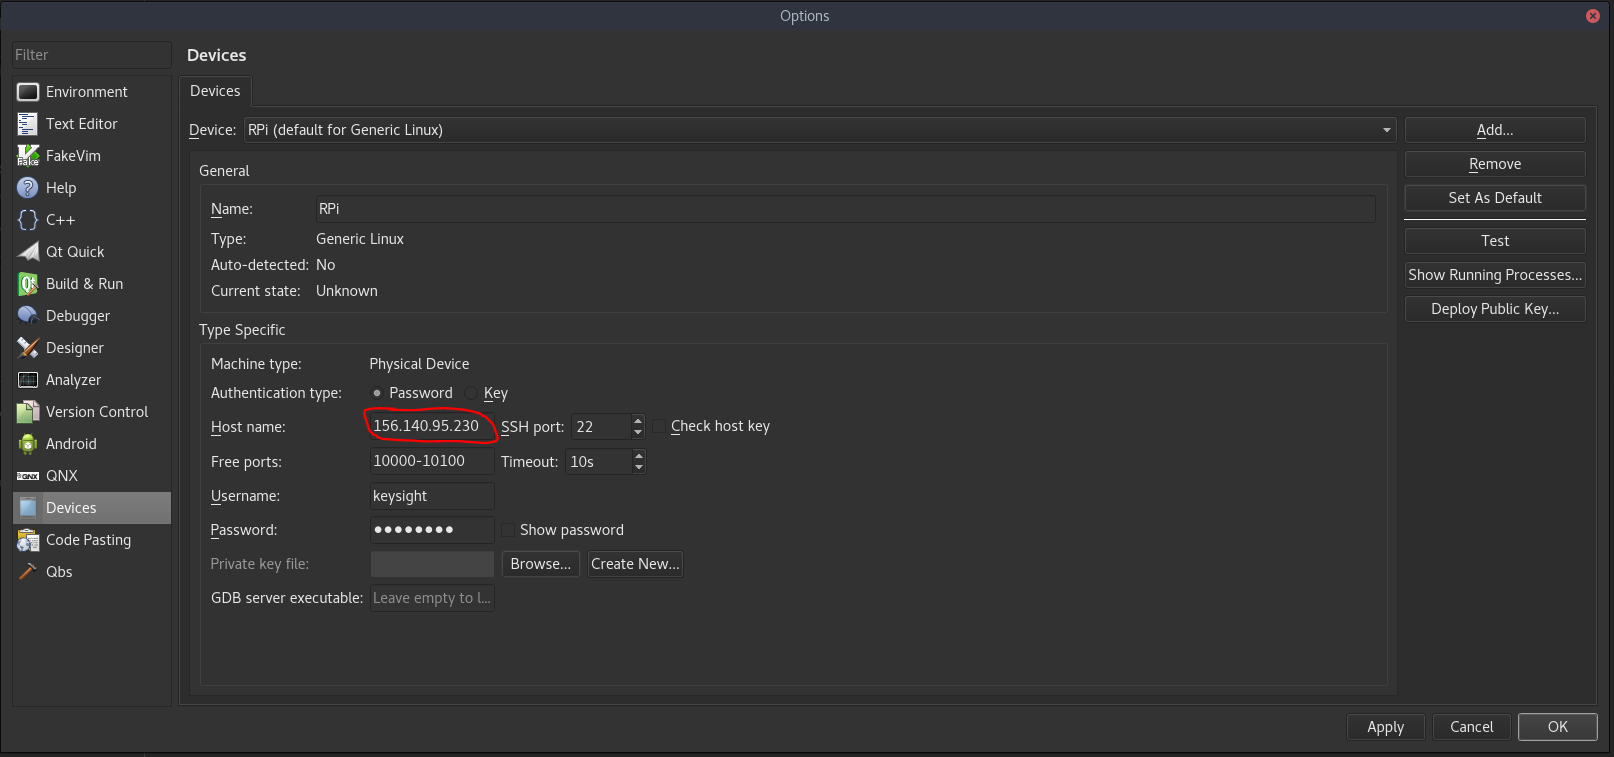
\includegraphics[scale=0.5]{pics/Qt_Options_Devices.png}
		\caption{Qt Creator Device Options}
		\label{Qt_Options_Devices}
	\end{figure}

After entering the IP address, click the \textbf{Test Button} on the right to make sure that Qt Creator can connect to the Raspberry Pi. You should see a dialog box similar to Figure \ref{Device_Test_Dialog}.

	\begin{figure}[H]
		\centering
		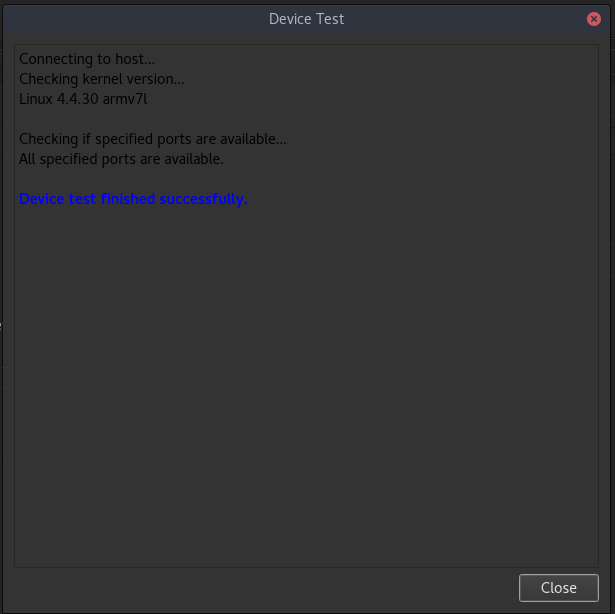
\includegraphics[scale=0.5]{pics/Device_Test_Dialog.png}
		\caption{Device Test Passed Message}
		\label{Device_Test_Dialog}
	\end{figure}

If the device passed the Raspberry Pi is connected to Qt Creator and ready for development. If it failed find a Keysight mentor and ask them to help setup Qt Creator.

%----------------------------------------------------------------------------------------
%	APPENDIX
%----------------------------------------------------------------------------------------

%\newpage
%\section{Appendix}

%\begin{enumerate}

	
%	\item[1. a.)] \lstinputlisting{../MATLAB/problem_1a.m}
	

%\end{enumerate}






%----------------------------------------------------------------------------------------


\end{document}